\documentclass{article}
\usepackage[utf8]{inputenc}
\usepackage{booktabs}
\usepackage[margin=1in]{geometry}
\usepackage{hyperref}
\hypersetup{
    colorlinks=true,
    linkcolor=blue,
    filecolor=magenta,      
    urlcolor=blue,
}

\urlstyle{same}

\title{Project 3 – Interactive Visualization using Tableau}
\author{Nathan McIntosh}
\date{Due October 13, 2020}

\usepackage{natbib}
\usepackage{graphicx}

\begin{document}

\maketitle

\section{Introduction}
The data set used for this project is the Kaggle \href{https://www.kaggle.com/kaggle/sf-salaries}{San Francisco city employee salary data}. It represents data on all the employees of the city from 2011 to 2014, some 148k rows. Each row contains a name, job title, and compensation in various forms for a given year. Detailed insight into compensation for government employees provides the public with confidence. It allows employees to know that they are, or are not, being fairly compensated for their work. It allows the public to freely ask questions like, ``how large is the pay gap between men and women?'', or ``are some employees being paid too much? Are some being paid too little?''. Detailed insight into government spending is critical for accountability and finding corruption. 
% ========================================
\section{Dataset}

\begin{table}[ht!]
\centering
\begin{tabular}{@{}rrrrrrrrr@{}}
\toprule
      & Id     & BasePay & OvertimePay & OtherPay & Benefits & TotalPay & TotalPayBenefits & Year   \\ \midrule
count & 148654 & 148045  & 148650      & 148650   & 112491   & 148654   & 148654           & 148654 \\
mean  & 74328  & 66325   & 5066        & 3649     & 25008    & 74768    & 93693            & 2013   \\
std   & 42913  & 42765   & 11454       & 8057     & 15402    & 50517    & 62794            & 1      \\
min   & 1      & -166    & 0           & -7059    & -34      & -618     & -618             & 2011   \\
25\%  & 37164  & 33588   & 0           & 0        & 11535    & 36169    & 44066            & 2012   \\
50\%  & 74328  & 65007   & 0           & 811      & 28629    & 71427    & 92404            & 2013   \\
75\%  & 111491 & 94691   & 4658        & 4236     & 35567    & 105839   & 132876           & 2014   \\
max   & 148654 & 319275  & 245132      & 400184   & 96571    & 567595   & 567595           & 2014   \\
category & nominal & quant & quant & quant & quant & quant & quant     & quant \\ \bottomrule
\end{tabular}
\end{table}

\section{Analytical Questions}
\begin{enumerate}
    \item Which jobs get the most and least base pay, as ordered by median base pay?
    \item Which jobs get the most overtime pay?
    \item Which jobs have the largest pay/benefits disparity?
    \item Do the number of employees in a job roll affect the median pay of that job?
    \item Which jobs had the greatest change in compensation from 2011 to 2014?
\end{enumerate}

\section{Design - design process, screenshot(s) of the different visualizations, and
explanation of overall dashboard}
In creating this dashboard, I wanted to examine questions 1, 2, 3, and 4. To create the first, I set the job title in the “columns” spot and $median(Base Pay)$ in the ``rows'', sorted by $median(Base Pay)$, and used a line as the marker to produce the plot in the top left. To examine count of job title against median total pay, I set $cnt(Job Title)$ as the columns, $median(Base Pay)$ as the rows, and set Job Title as a ``detail'', which created the scatter plot seen in the top right. Because most of the jobs have less than 100 people performing them, and a few have almost 10,000, I used a log scale better spread the data out. To see the top ten jobs by overtime pay, I set job title as columns, and median overtime pay as the rows, and sorted the data. Finally, to visualize the pay/benefits disparity, I created a calculated field named BasePayBenefitsDiff, calculated by $median((Base Pay-Benefits)/Base Pay)$. This calculated field is 0 when there is no difference between Base Pay and Benefits, and it is 1 when Benefits is 0, or is negligibly small in comparison to Base Pay. I then placed this newly calculated field as the columns, and job title as the rows, and sorted. The final result is the dashboard seen below.

\begin{figure}[h!]
\centering
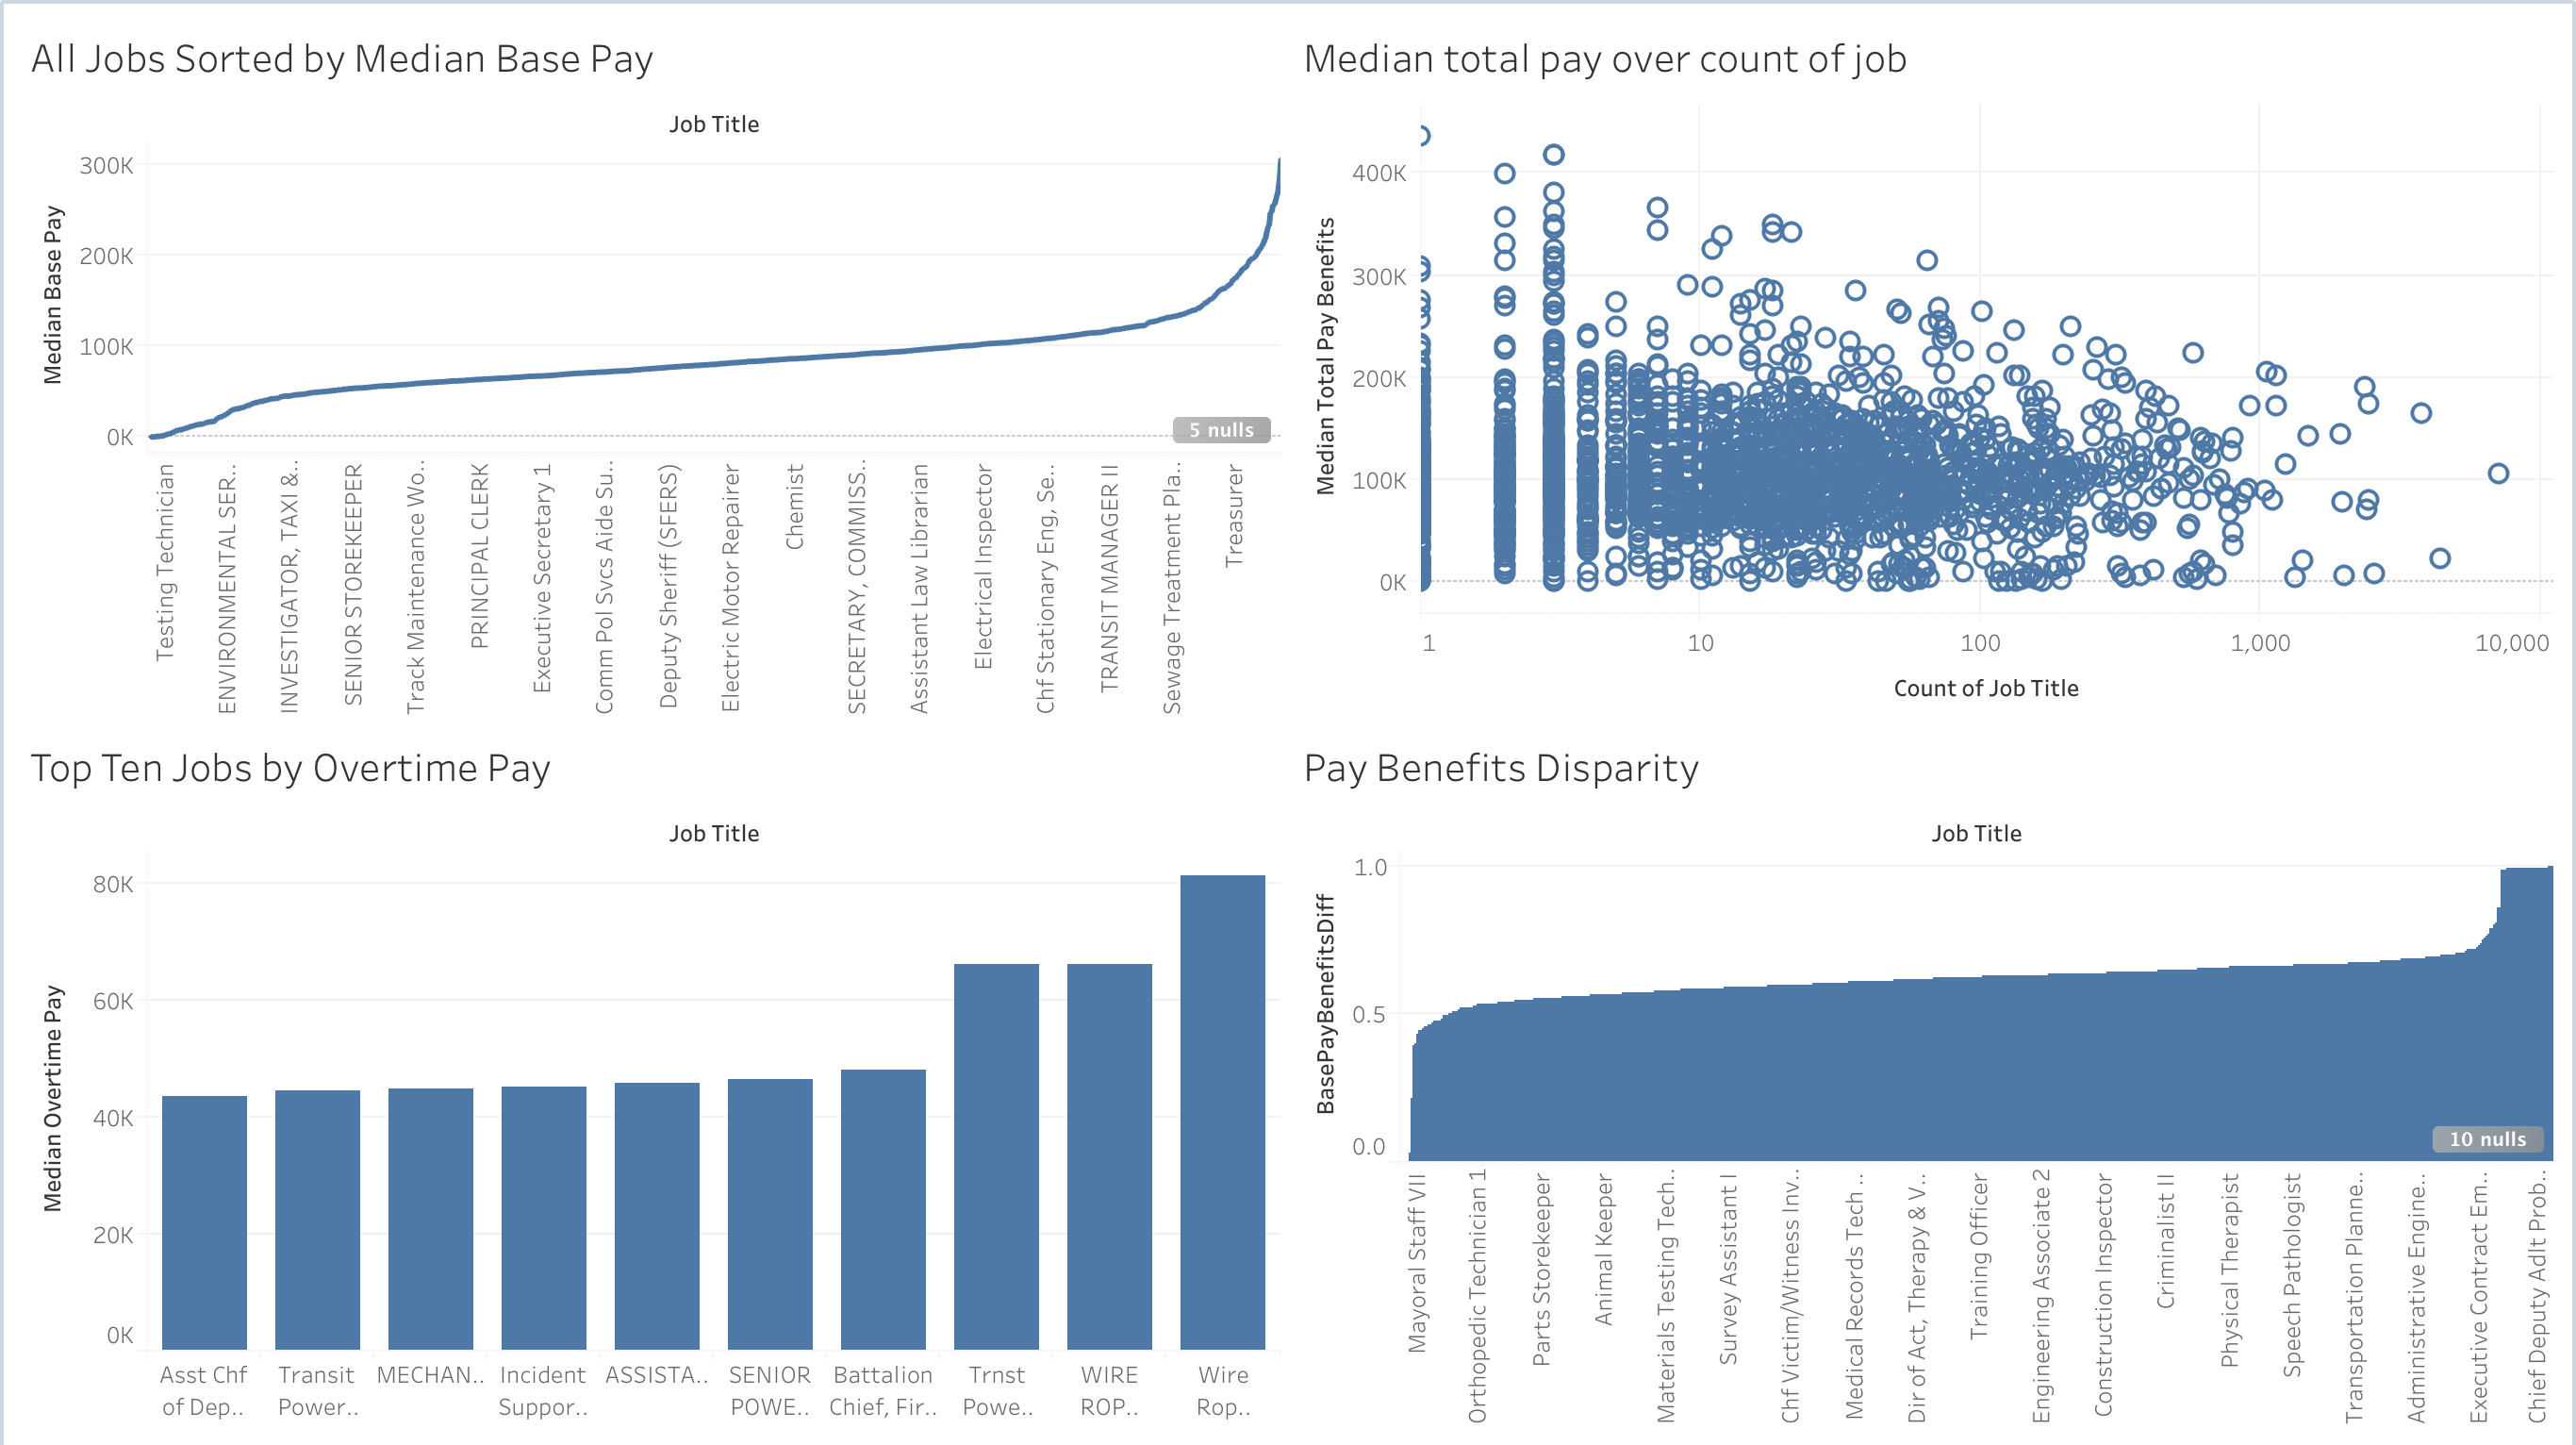
\includegraphics[scale=0.35]{dashboard_screenshot.png}
\caption{Screen Shot of the Dashboard}
\label{fig:dashboard}
\end{figure}

\section{Discussion - explain how the dashboard answers some of the analytical questions}

Question 1 was which jobs get the most and least base pay, as ordered by median base pay? The top left plot answers this question by showing us the total range of base pays that employees of the city receive. The plot shows that some receive nothing for their work, most receive less than \$100k, and a few receive over \$300k. 

Question 2 was which jobs get the most overtime pay? The bottom left graphic clearly answers this question with its bar chart of said top ten jobs as ranked by overtime pay. The names are listed at the bottom of each bar, and the bar heights show the median overtime pay for that profession. 

Question 3 was which jobs have the largest pay/benefits disparity? The bottom right plot answers this with a bar chart of BasePayBenefitsDiff for all professions. The interactive nature allows the user to selectively view jobs. 

Question 4 was do the number of employees in a job roll affect the median pay of that job? The top right plot shows that this is unlikely to be true. There is no clear trend here one way or another. 

\end{document}
